
\subsection{Parameters calculation}


\noindent
RHF corresponds to the weight average of hydride length multiplied by a weighting factor. The formula employed is described below:


\begin{figure}[h] %  figure placement: here, top, bottom, or page
    \raggedleft
    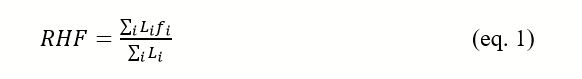
\includegraphics[width=4.5in]{Figures/2-Parameters/RHF.JPG}
    \label{fig:my_label}
\end{figure}


\noindent
Where $L_i$ is the length of each hydride and $f_i$ is the weighting factor, a parameter that has different values depending on the hydrides orientation. Hydrides with orientations between 0-40° to the transverse direction have a $f_i$ of 0, when the orientation is between 40° and 65°, the $f_i$ is 0.5, and hydrides with an orientation of 65–90° have a $f_i$ of 1 \cite{COLAS2013586}. 

\noindent
To calculate the HCC, a rectangular area in the micrograph of the alloy is separated, and the length of each radial hydride in that area is measured. The formula applied is shown below:


\begin{figure}[h] %  figure placement: here, top, bottom, or page
    \raggedleft
    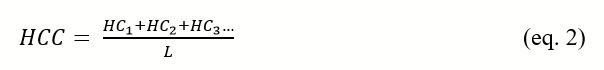
\includegraphics[width=4.3in]{Figures/2-Parameters/HCC.JPG}
    \label{fig:my_label}
\end{figure}
\noindent
Where $HC_i$ is the length of each radial hydride and L is the height of the selected rectangle to measure \cite{SIMON2021152817}.

\noindent
To calculate the RHCF, the length of each radial hydride in a section of the cladding is measured. This time, the section will have a length of 150 µm along the arc length of the cladding, and the width will be all the cladding thickness. The formula applied in this case is:

\begin{figure}[h] %  figure placement: here, top, bottom, or page
    \raggedleft
    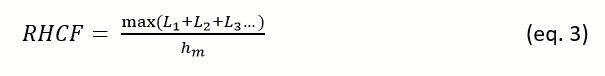
\includegraphics[width=4.5in]{Figures/2-Parameters/RHCF.JPG}
    \label{fig:my_label}
\end{figure}

\vspace{150}
\noindent
Where $L_i$ is the length of each radial hydride within the 150 µm of arc length, and $h_m$ is the cladding thickness \cite{SIMON2021152817}.